
 
  In this section we explore the sharpening mechanism empirically.
  We consider inference-time experiments that demonstrate that self-improvement through sharpening is possible, as well as training-time experiments that successfully amortize the cost of self-improvement, thereby avoiding computational overhead at inference time.  We first describe the general experimental setup, then turn to the results of our experiments.

\subsection{Experimental Setup}

We experiment with sharpening using the following models, all of which (except for \gptthree) are available on \url{https://huggingface.co}; we provide HuggingFace model identifiers below.
\begin{enumerate}
\item Phi models: We use several models from the Phi family~\citep{abdin2024phi}, specifically \phithreemini (``microsoft/Phi-3-mini-4k-instruct''), \phithreesmall (``microsoft/Phi-3-small-8k-instruct''), \phithreemedium (``microsoft/Phi-3-medium-4k-instruct''), and \phithreefivemini (``microsoft/Phi-3.5-mini-instruct''). 
\item \llamathree (``meta-llama/Llama-3.2-3B-Instruct'')~\citep{dubey2024llama}.
\item \mistral (``mistralai/Mistral-7B-Instruct-v0.3'')~\citep{jiang2023mistral}.
\item \gptthree~\citep{brown2020language}: We access this model via the OpenAI API.
\item \llamagame (``OhCherryFire/llama2-7b-game24-policy-hf''): We use the model of \iftoggle{workshop}{\cite{wan2024alphazero}}{\citet{wan2024alphazero}}, which is a Llama-2 model finetuned on the \gametwentyfour task \citep{yao2024tree}. We use this model only for experiments with \gametwentyfour. 
\end{enumerate}

We consider the following tasks:

\begin{enumerate}
      \item \gsm: We use the above models to generate responses to prompts from the GSM-8k dataset \citep{cobbe2021training} where the goal is to generate a correct answer to an elementary school math question. For inference-time experiments, we take the first 256 examples from the test set in the ``main'' subset.\footnote{\url{https://huggingface.co/datasets/openai/gsm8k}.} %
    \item \mathdataset: We use the above models to generate responses to prompts from the \mathdataset dataset \citep{hendrycks2021measuring}, which consists of more difficult math questions.  For inference-time experiments, we consider ``all'' subsets and take the first 256 examples of the test set where the solution matches the regular expression \verb|(\d*)|.\footnote{\url{https://huggingface.co/datasets/lighteval/MATH}.}  %
    \item \prontoqa: We use the above models to generate responses to prompts from the \prontoqa dataset \citep{saparov2023language}, which consists of chain-of-thought-style reasoning questions with boolean answers.  For inference-time experiments, we take the first 256 examples from the training set.\footnote{\url{https://huggingface.co/datasets/longface/prontoqa-train}.} %
    \item \mmlu: We use the above models to generate responses to prompts from three subsets of the \mmlu dataset \citep{hendrycks2020measuring}, specifically \texttt{college\_biology} (Bio), \texttt{college\_physics} (Phys), and \texttt{college\_chemistry} (Chem), all of which consist of multiple choice questions.\footnote{\url{https://huggingface.co/datasets/cais/mmlu}.} For inference-time experiments, we take the first 256 examples of the test set for each subset. 
    \item \gametwentyfour: We use only the model of \iftoggle{workshop}{\cite{wan2024alphazero}}{\citet{wan2024alphazero}} (i.e., \llamagame), on the \gametwentyfour task \citep{yao2024tree}.  The prompts are four numbers and the goal is to combine the numbers with standard arithmetic operations to reach the number `24.'  For inference-time experiments, we use both the train and test splits of the dataset.\footnote{\url{https://github.com/princeton-nlp/tree-of-thought-llm/tree/master/src/tot/data/24}}  %
    \end{enumerate}

    All of our experiments were run on 40G NVIDIA A100 GPUs, 192G AMD MI300X GPUs, or through the OpenAI API.


    \subsection{Validation of Inference-Time Sharpening}\label{ssec:inference}

    We first validate the sharpening mechanism (i.e., the phenomenon that responses from a model with high self-reward $\rself$ enjoy high performance on downstream tasks) through inference-time experiments, focusing on the maximum likelihood self-reward. For each (model, task) pair, we sample $N$ generations per prompt with temperature 1 and return the best of the $N$ generations according to the \mlsharp self-reward function $\rself(y\mid{}x)=\log\piref(y\mid{}x)$; we compare against greedy decoding as a baseline, whose accuracy is displayed in \Cref{sfig:bon-greedy}.




\paragraph{Implementation details}
For all models and datasets except for \gametwentyfour, we used 1-shot prompting to ensure that models conform to the desired output format and to elicit chain of thought reasoning (for \gametwentyfour we do not provide a demonstration in the prompt). We set the maximum length of decoding to be $512$ tokens. We used 10 seeds for all (model, task) pairs with a maximum value of $N=50$ in \BestofN sampling. We simulated $N$ responses for $N<50$ by subsamplng the 50 generated samples. For \BestofN sampling, we always use temperature $1.0$. Since greedy decoding is a deterministic strategy, there is no need to average over multiple seeds for each (model, task) pair. In all experiments, we collect both the responses and their log-likelihoods under the \emph{reference model} (i.e., the original model from which samples were generated). 

\paragraph{Results}
We display our findings in \Cref{fig:validation}(a) and in \Cref{fig:BoN-inference-granular}; because we only consider a single model for \gametwentyfour, we separate the results for this task into \Cref{fig:game24_inf}. We visualize performance---measured through normalized accuracy improvement over greedy decoding. We also visualize log-likelihoods (under $\piref$) of the selected responses in \cref{fig:BoN-inference-logprobs}. We find that:
\begin{enumerate}
\item Across all (model, task) pairs, inference-time \BestofN
  sharpening (using $\rself(y\mid{}x)=\log\piref(y\mid{}x)$) improves
  over na{\"i}ve sampling with temperature 1.0.
\item For all datasets, \BestofN sharpening improves upon standard \emph{greedy decoding}, for at least one model.
  \item Analogously, for every model, there is at
  least one dataset for which \BestofN sharpening improves over greedy
  decoding.
\end{enumerate}

We further explore the relationship between sequence-level log-probabilities and generation quality in \Cref{fig:distributions}, where we plot the empirical distributions of responses sampled with temperature 1 from the base model for a variety of model-dataset pairs, conditioned on whether or not the response is correct. We find that \emph{the distribution of log probabilities conditioned on correctness stochastically dominates the distribution conditioned on incorrectness} in each (model, task) pair evaluated, which provides more evidence that maximum likelihood sharpening represent a reasonable self-improvement target.

We mention several other observations from the experiments. First, in most cases, performance and log-likelihood saturate at relatively small values of $N$, typically around 10 or 20. This suggests that significant improvements can be obtained with relatively low computational overhead. Second, in some cases, performance can degrade as $N$ increases. We found that this happens for two reasons: (1) the performance of the reference model is poor and so $\rself$ does not provide a good signal (e.g., with \llamathree) and (2) the \BestofN criteria selects for short responses, which have higher log-likelihood but cannot leverage the computational and representational benefits of chain-of-thought, thereby yielding worse performance (e.g., with \gptthree on \gsm). 


    \begin{figure}[tp]
    \centering
    \subfigure[]{
    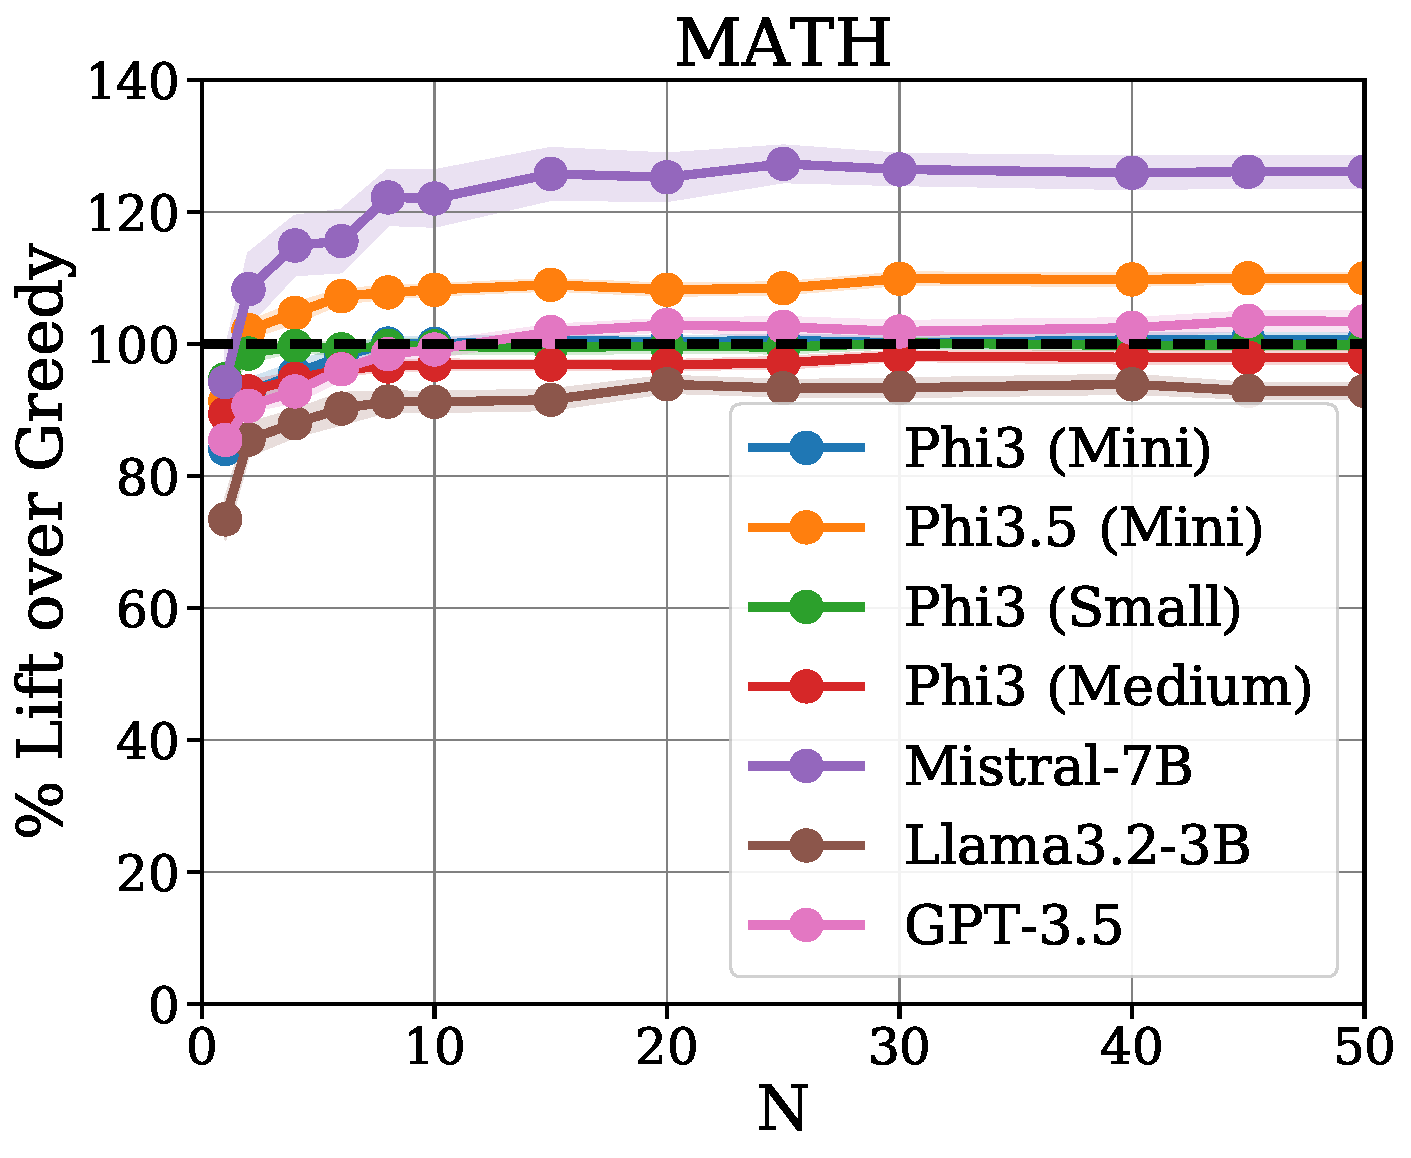
\includegraphics[width=0.45\textwidth]{figs/BoN-math-improvement.pdf}
    }
    \hfill
    \subfigure[]{
    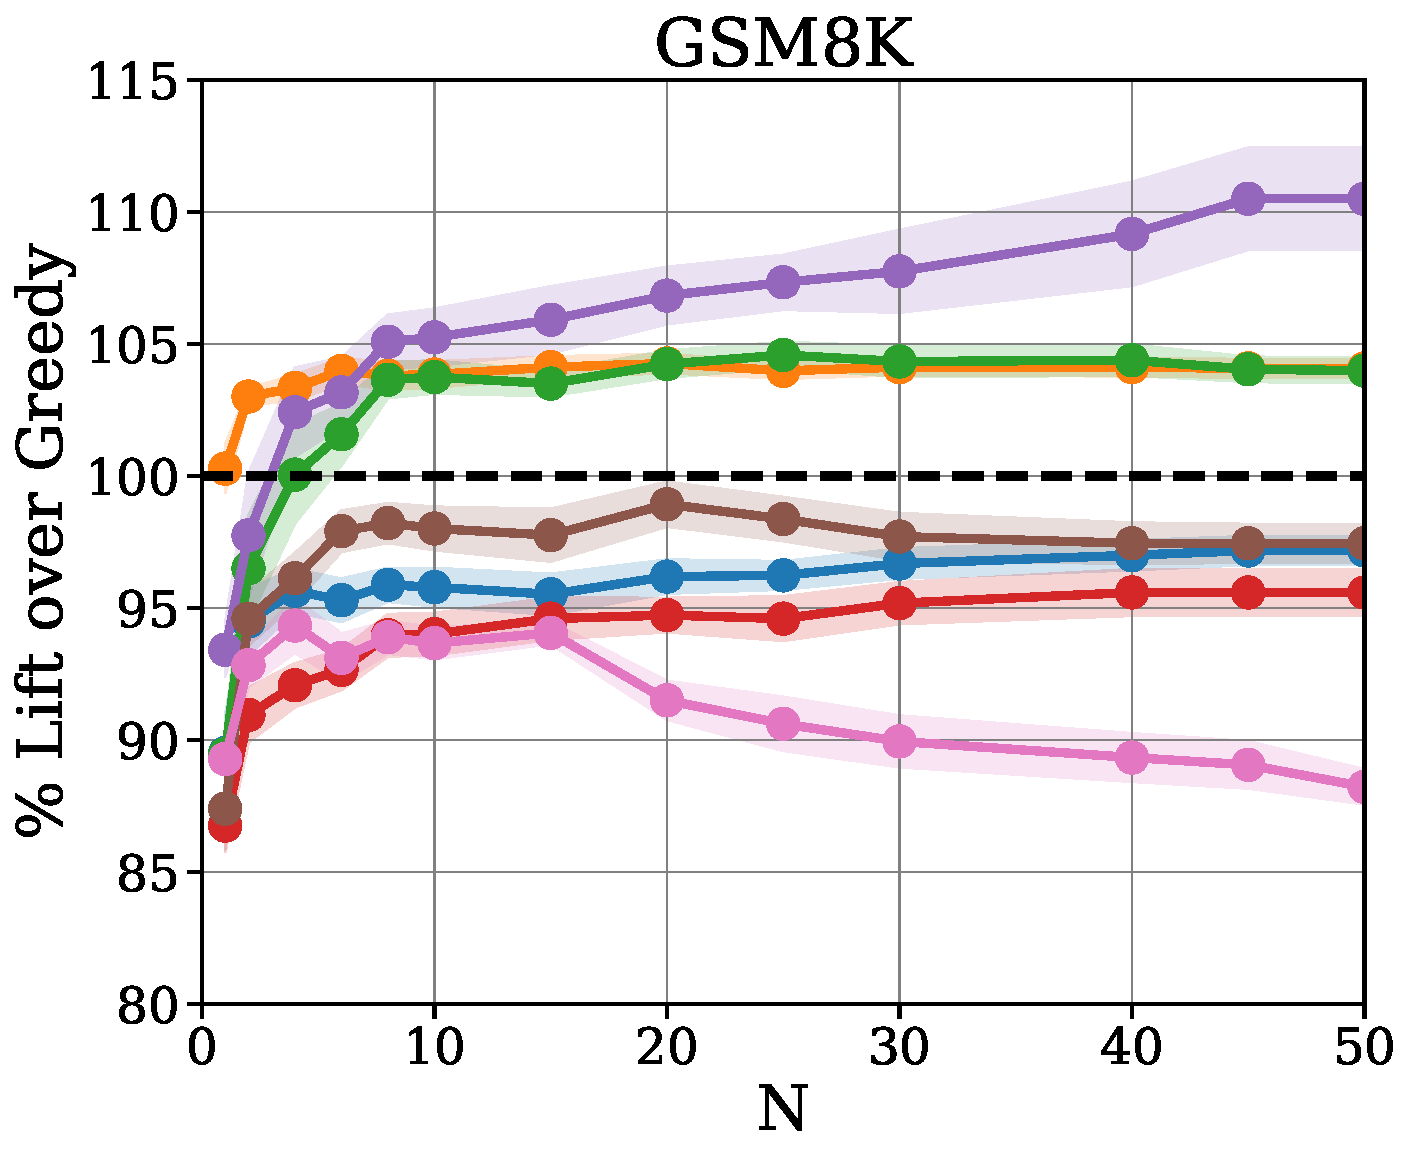
\includegraphics[width=0.45\textwidth]{figs/BoN-gsm8k-improvement.pdf}
    }
    \\
    \subfigure[]{
    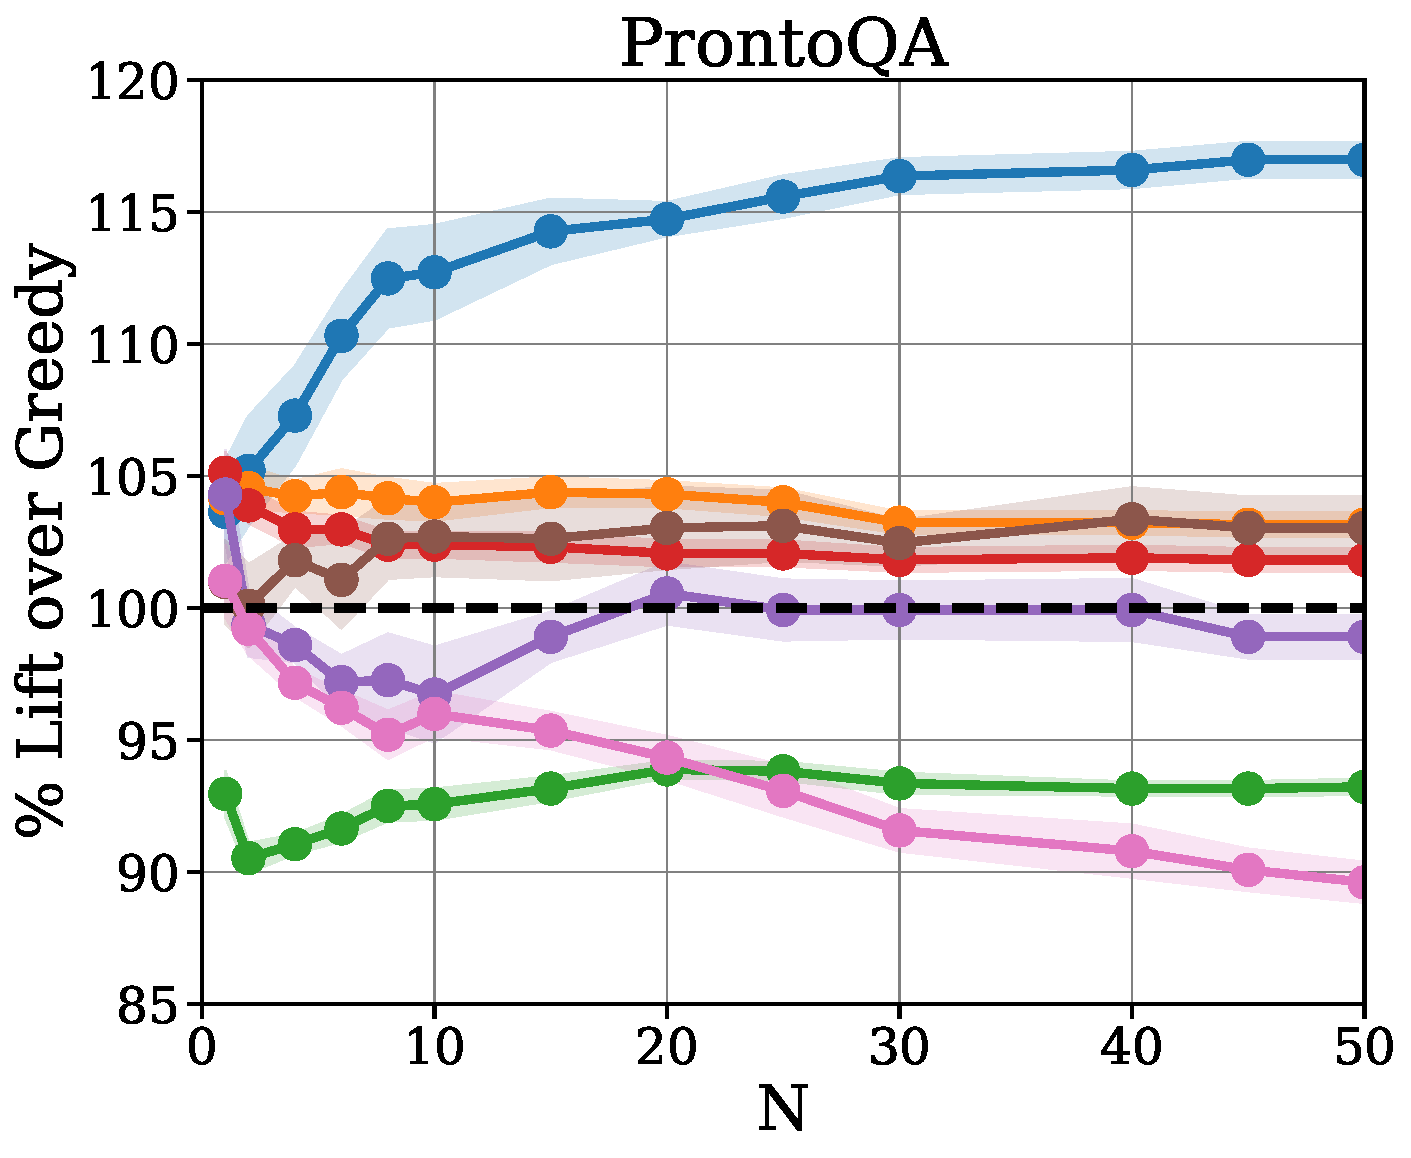
\includegraphics[width=0.45\textwidth]{figs/BoN-prontoqa-improvement.pdf}
    }
    \hfill
    \subfigure[]{
    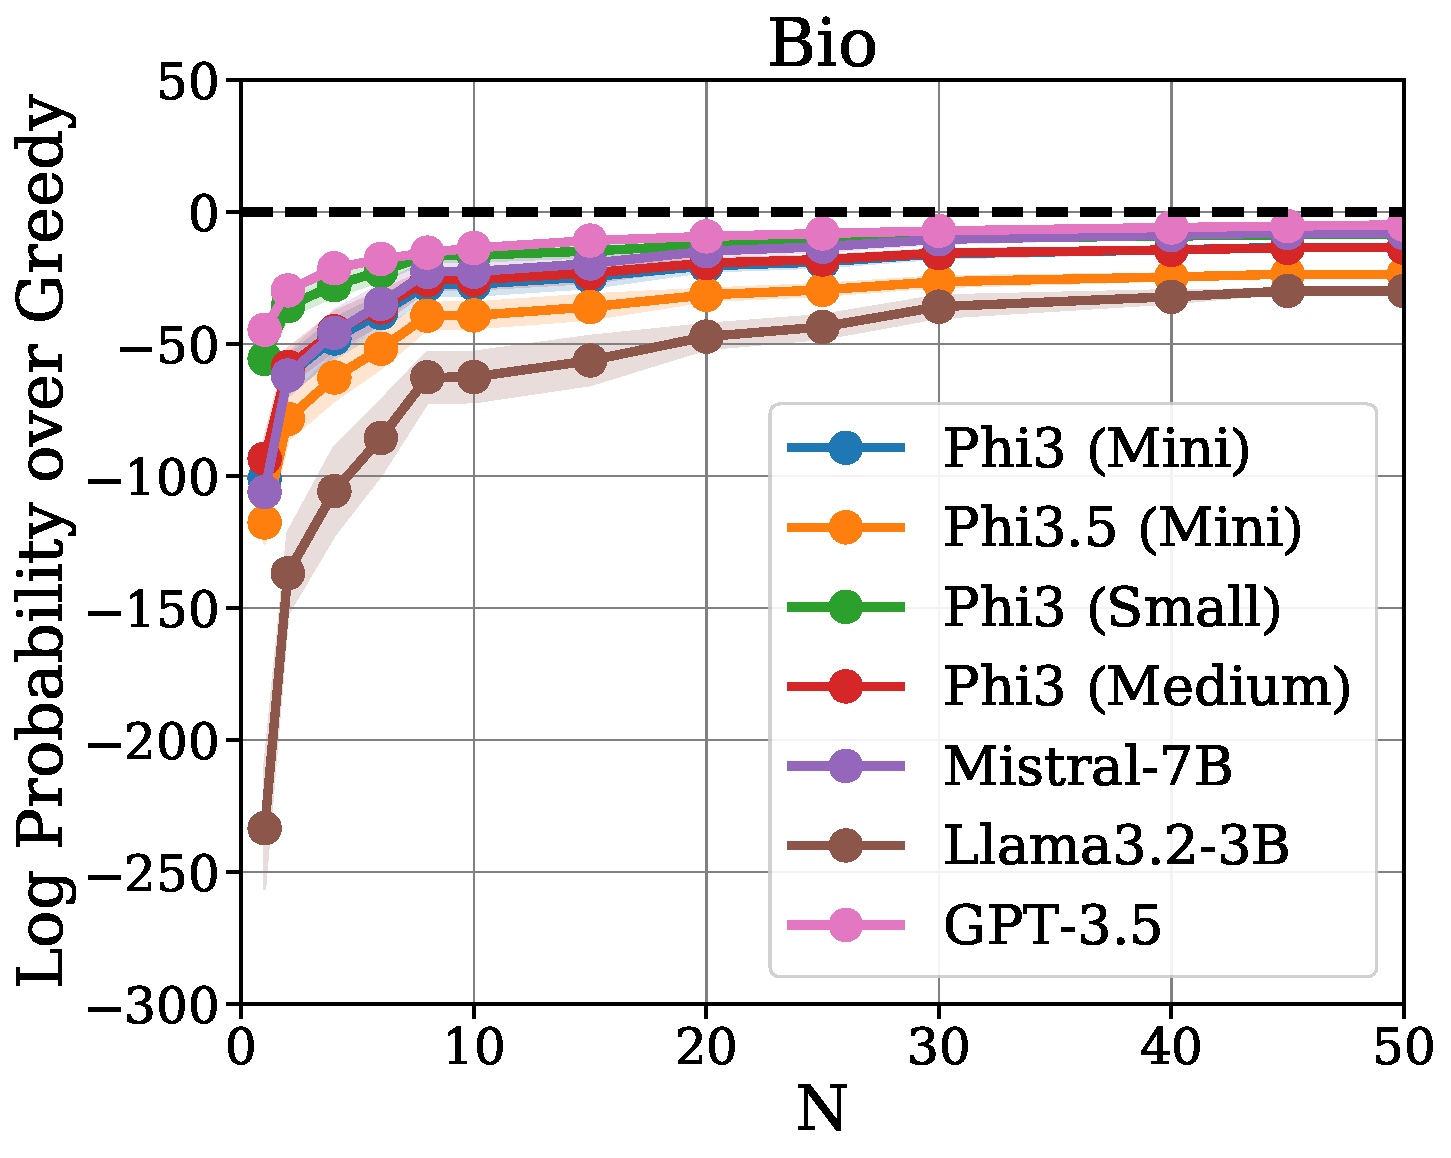
\includegraphics[width=0.45\textwidth]{figs/BoN-mmlu-bio-logprobs.pdf}
    }
    \\
    \subfigure[]{
    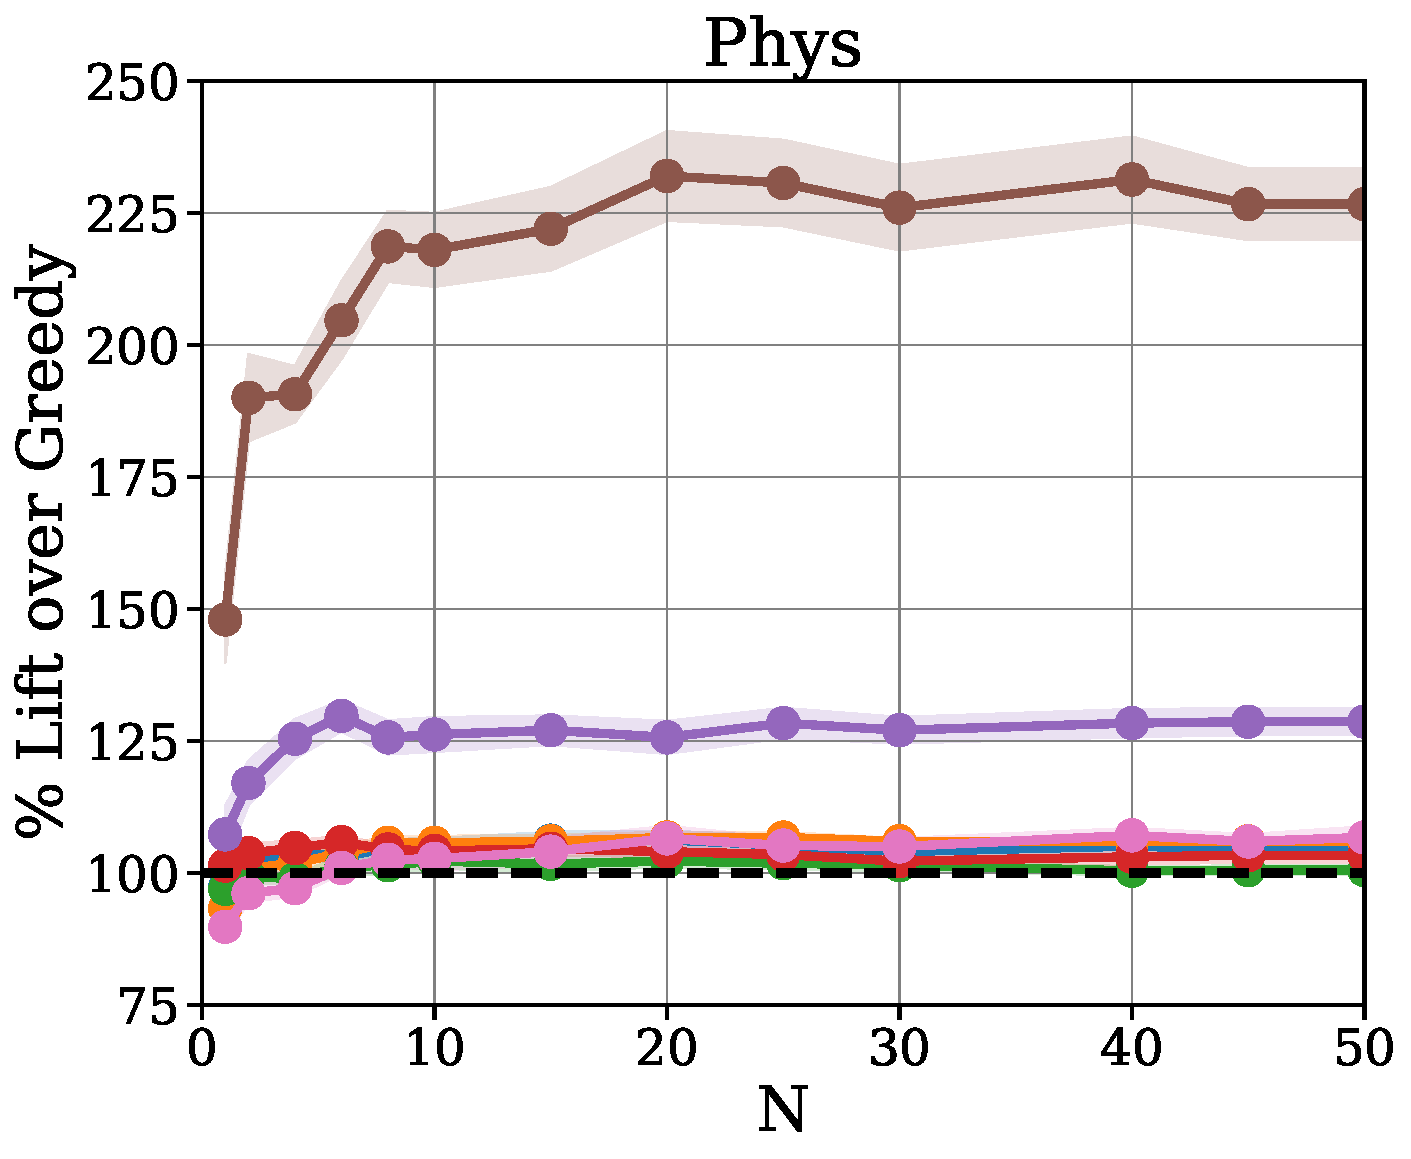
\includegraphics[width=0.45\textwidth]{figs/BoN-mmlu-phys-improvement.pdf}
    }
    \hfill
    \subfigure[]{
    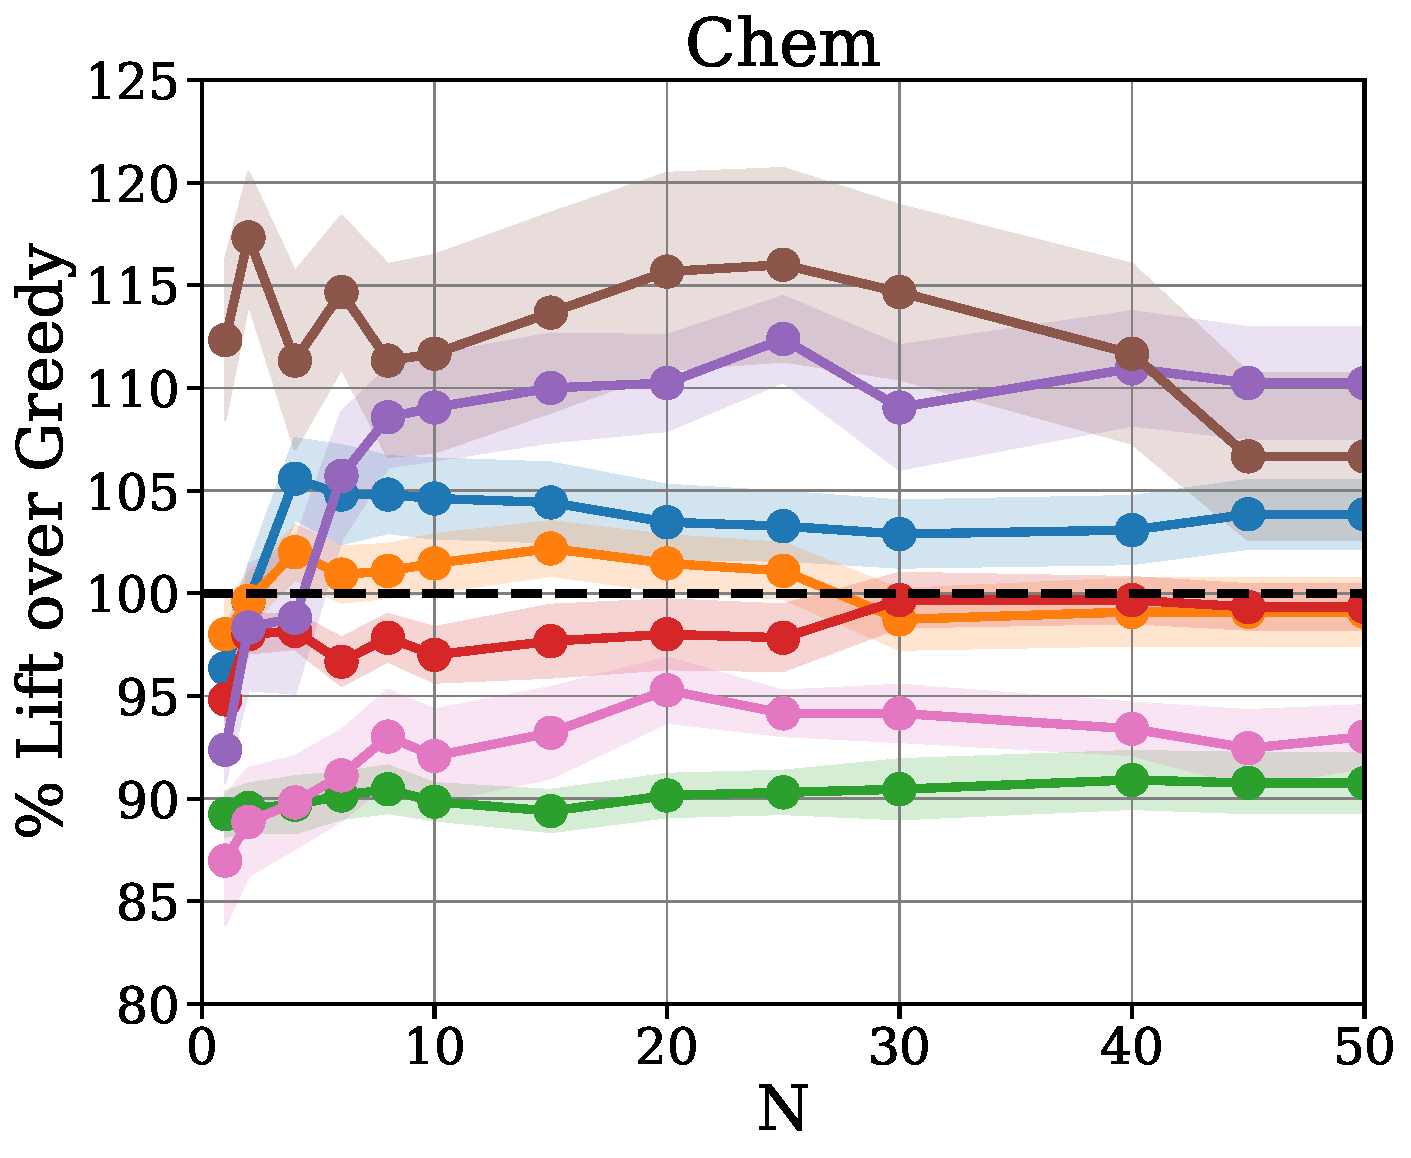
\includegraphics[width=0.45\textwidth]{figs/BoN-mmlu-chem-improvement.pdf}
    }
    \caption{Percent lift in accuracy of inference-time BoN-sharpening over greedy decoding in each task as $N$ is varied.  For many task-model pairs, the accuracy improves as $N$ increases, demonstrating the efficacy of maximum likelihood sharpening.}
    \label{fig:BoN-inference-granular}
\end{figure}



\subsection{Inference-Time Sharpening with other Self-Reward Functions}
Although we focus on $\rself(y \mid{}x) = \log\piref(y \mid{}x)$ throughout the paper, the sharpening framework is significantly more general.\footnote{Although we do not experiment with model-as-judge approaches~\citep[e.g.,][]{huang2022large}, which obtain self-reward by re-prompting, we note that they can be cast in the sharpening framework by simply defining the self reward $\rself(y \mid{} x)$ to be the output of the model when prompted with a verification/scoring prompt, the original prompt $x$ and the candidate response $y$.} As such, we experiment with inference-time sharpening for other choices for $\rself$:\loose
\begin{enumerate}
  \item Length-normalized log-likelihood: $\rself(y \mid{}x) = \frac{1}{|y|} \log\piref(y \mid{}x)$ where $|y|$ is the length, in tokens, of the response.
  \item Majority (self-consistency): All datasets except \gametwentyfour have multiple-choice, boolean, or numerical answers. Although we allow responses to contain chain-of-thought tokens, we can extract the answer from each response and use the most-frequently-occuring answer. This can be seen as a sample-based approximation to the following self-reward function: $\rself(y\mid{}x) = \sum_{y': y'_{\texttt{ans}}=y_{\texttt{ans}}} \piref(y'\mid{}x)$, where $y_{\texttt{ans}}$ are the ``answer'' tokens in the full response $y$. 
\end{enumerate}
Finally, as a skyline we consider the \emph{coverage} criterion~\citep{brown2024large}, where we simply check if any of the sampled responses corresponds to the correct answer. This criterion is a skyline and does not fit into sharpening framework, as it uses knowledge of the ground truth (external) task reward function. 

Results are displayed in \Cref{fig:other_rewards}. For length-normalized log-likelihood (a) and majority (b), we see qualitatively similar behavior to (unnormalized) log-likelihood: inference-time sharpening via these self-reward functions offers improvement over both vanilla (temperature 1.0) sampling and greedy decoding. In both cases, the improvements are generally larger than those obtained with log-likelihood. Finally, examining the coverage criteria, we see that with $N=50$ samples, all of the models almost always produce a correct answer on all tasks, raising the possibility of other self-reward functions that further improve performance.


\begin{figure}[t]
    \centering
    \subfigure[]{
        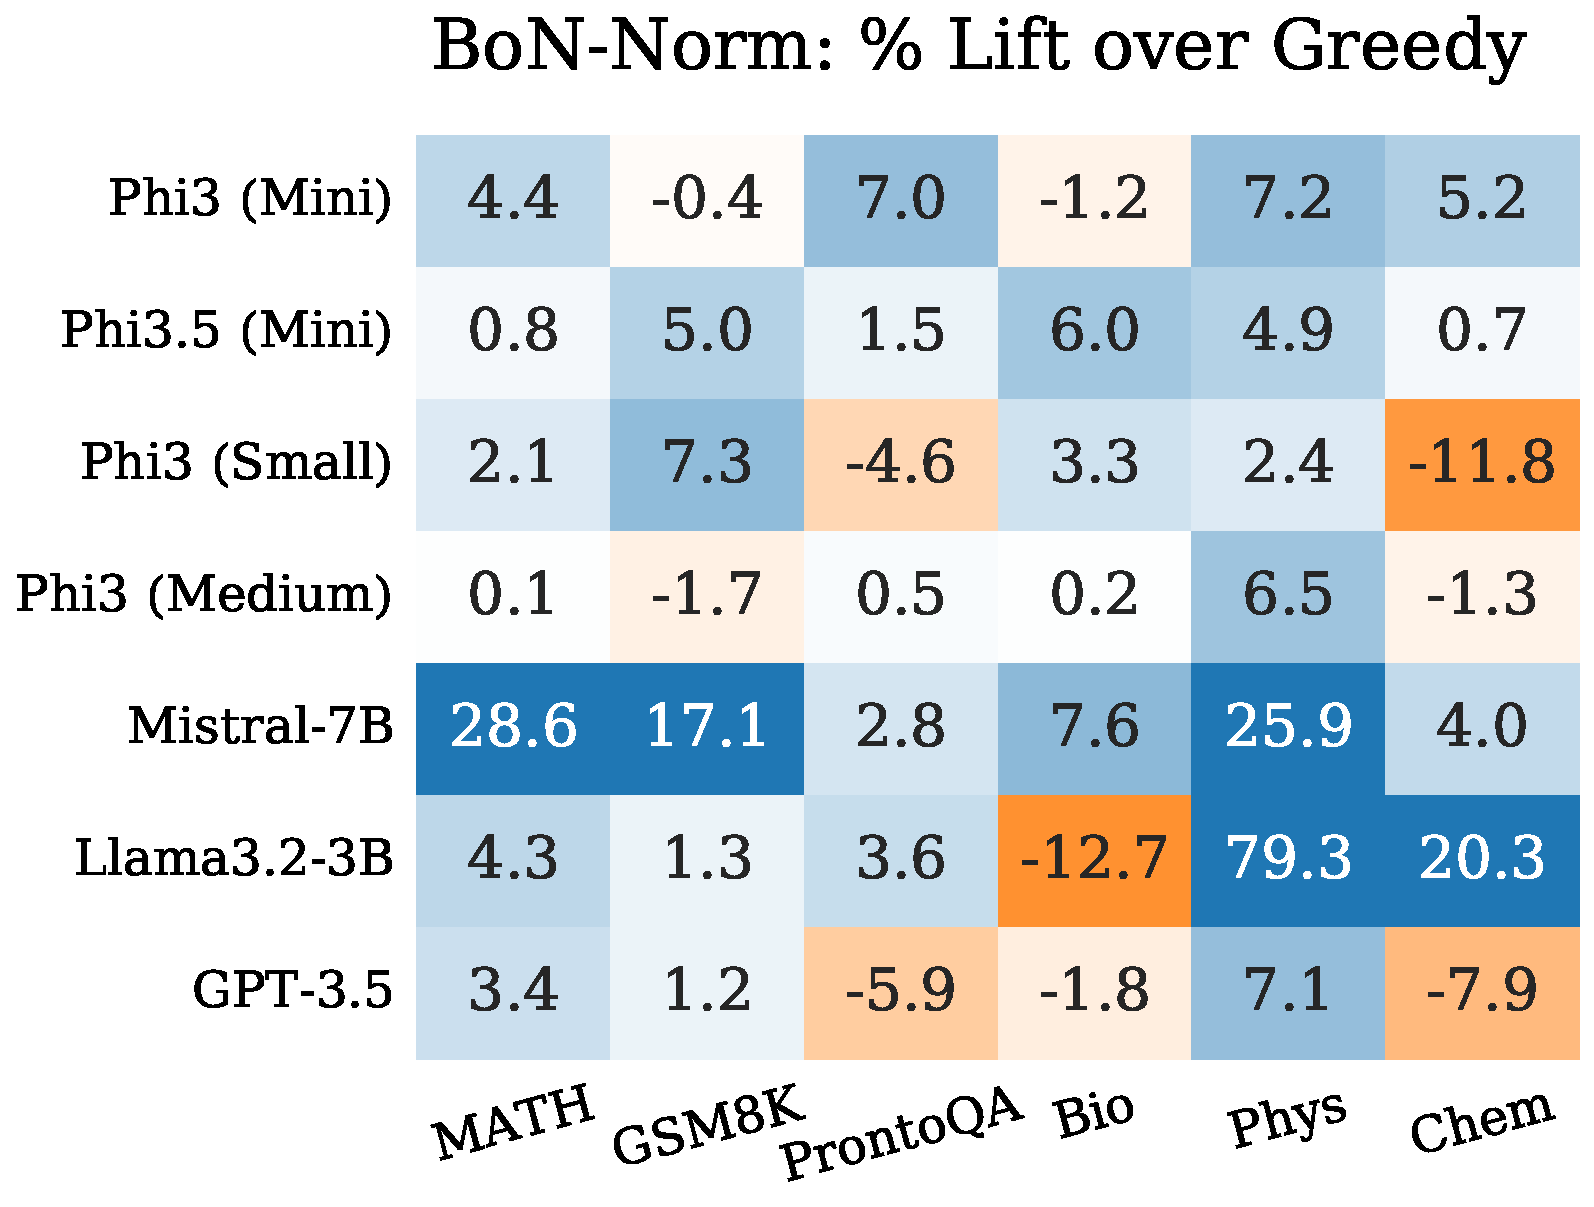
\includegraphics[width=0.45\textwidth]{figs/BoN-Normalized-Colored-Table.pdf}
        \label{sfig:bon-normalized-improvement} 
    }
    \hfill \subfigure[]{
        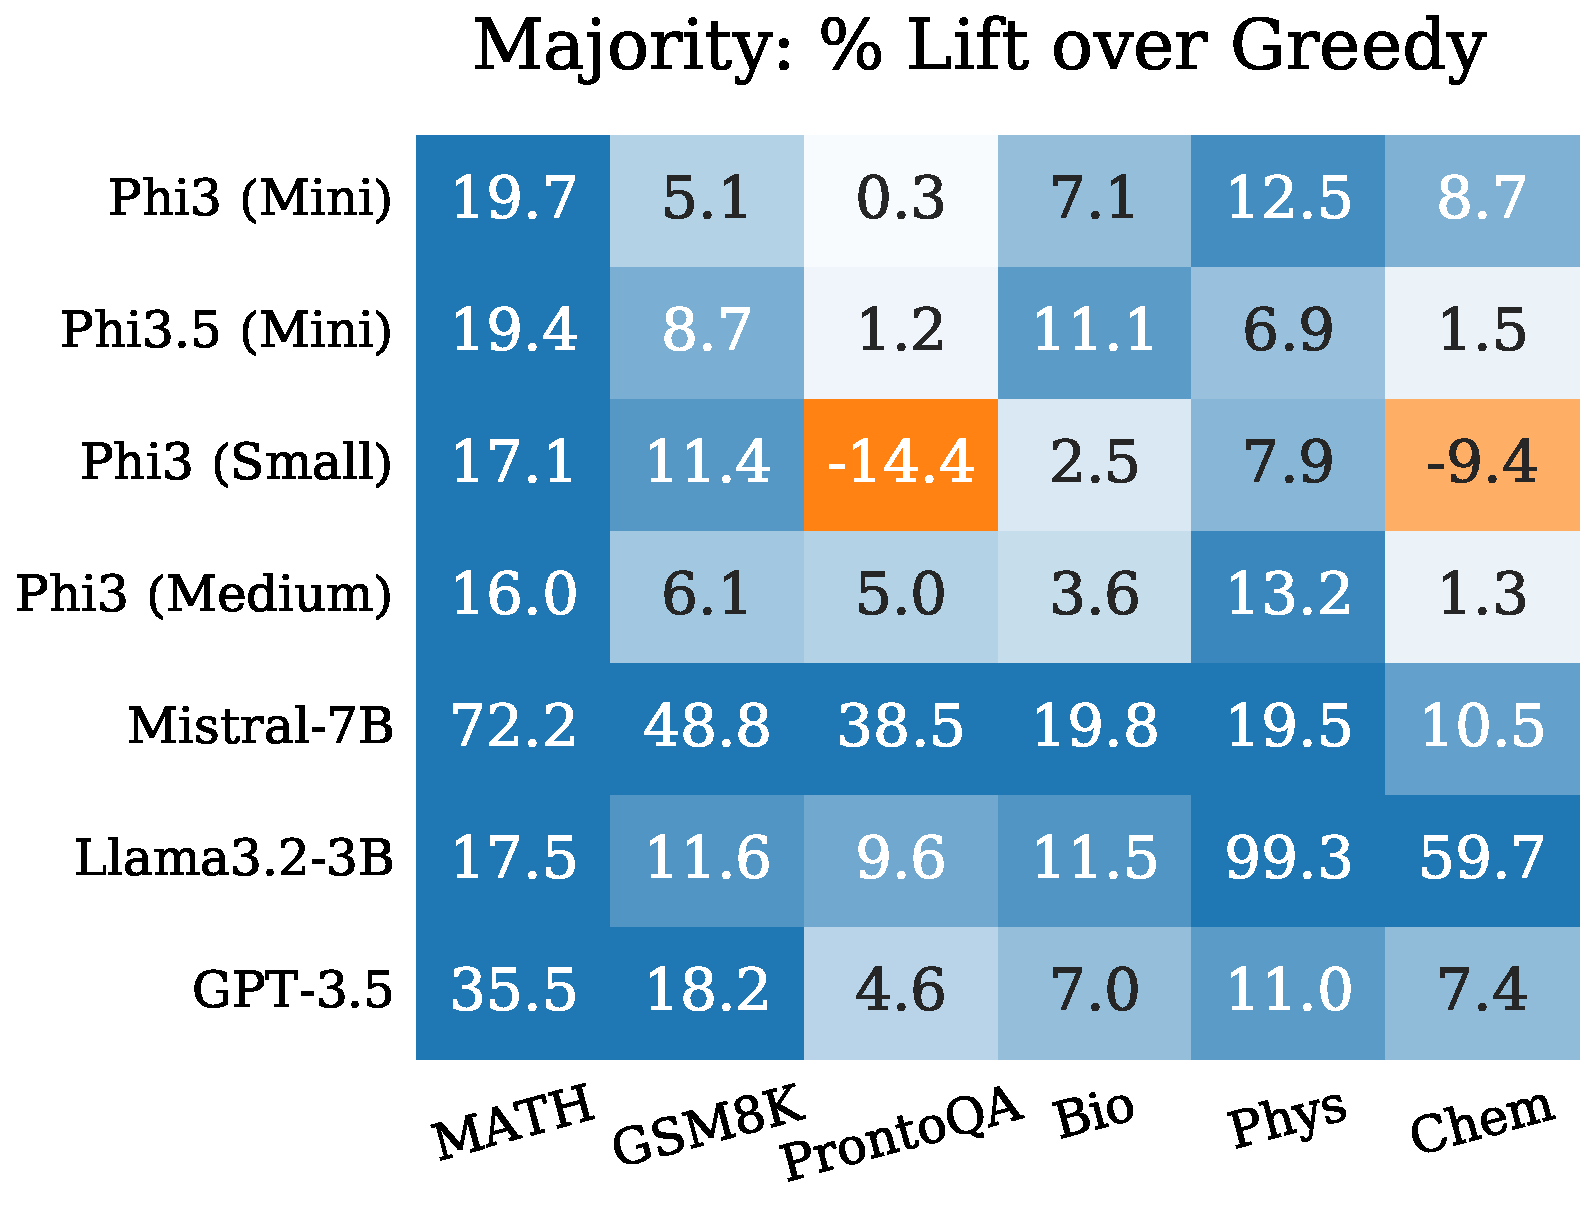
\includegraphics[width=0.45\textwidth]{figs/BoN-Majority-Colored-Table.pdf}
        \label{sfig:bon-majority-improvement}
    } \\
  
    \subfigure[]{
        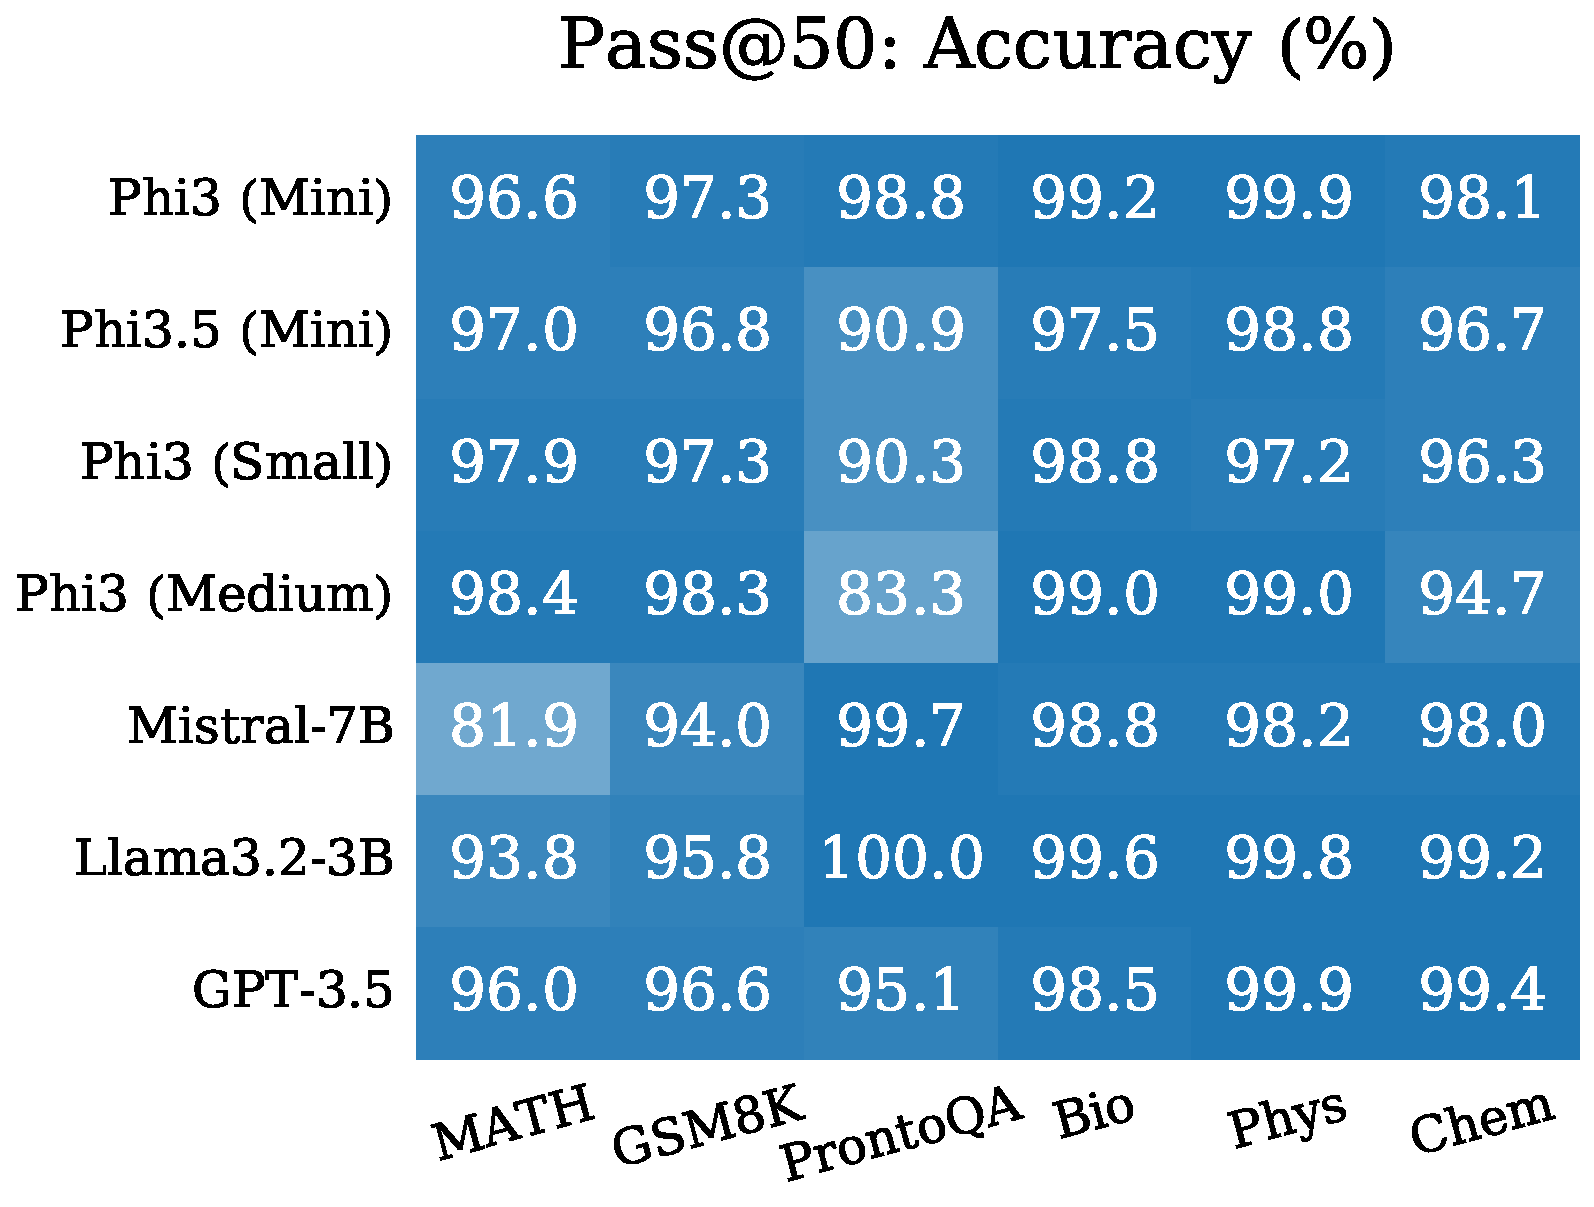
\includegraphics[width=0.45\textwidth]{figs/BoN-Coverage-Colored-Table.pdf}
        \label{sfig:bon-coverage}
    }
    \hfill
    \subfigure[]{
        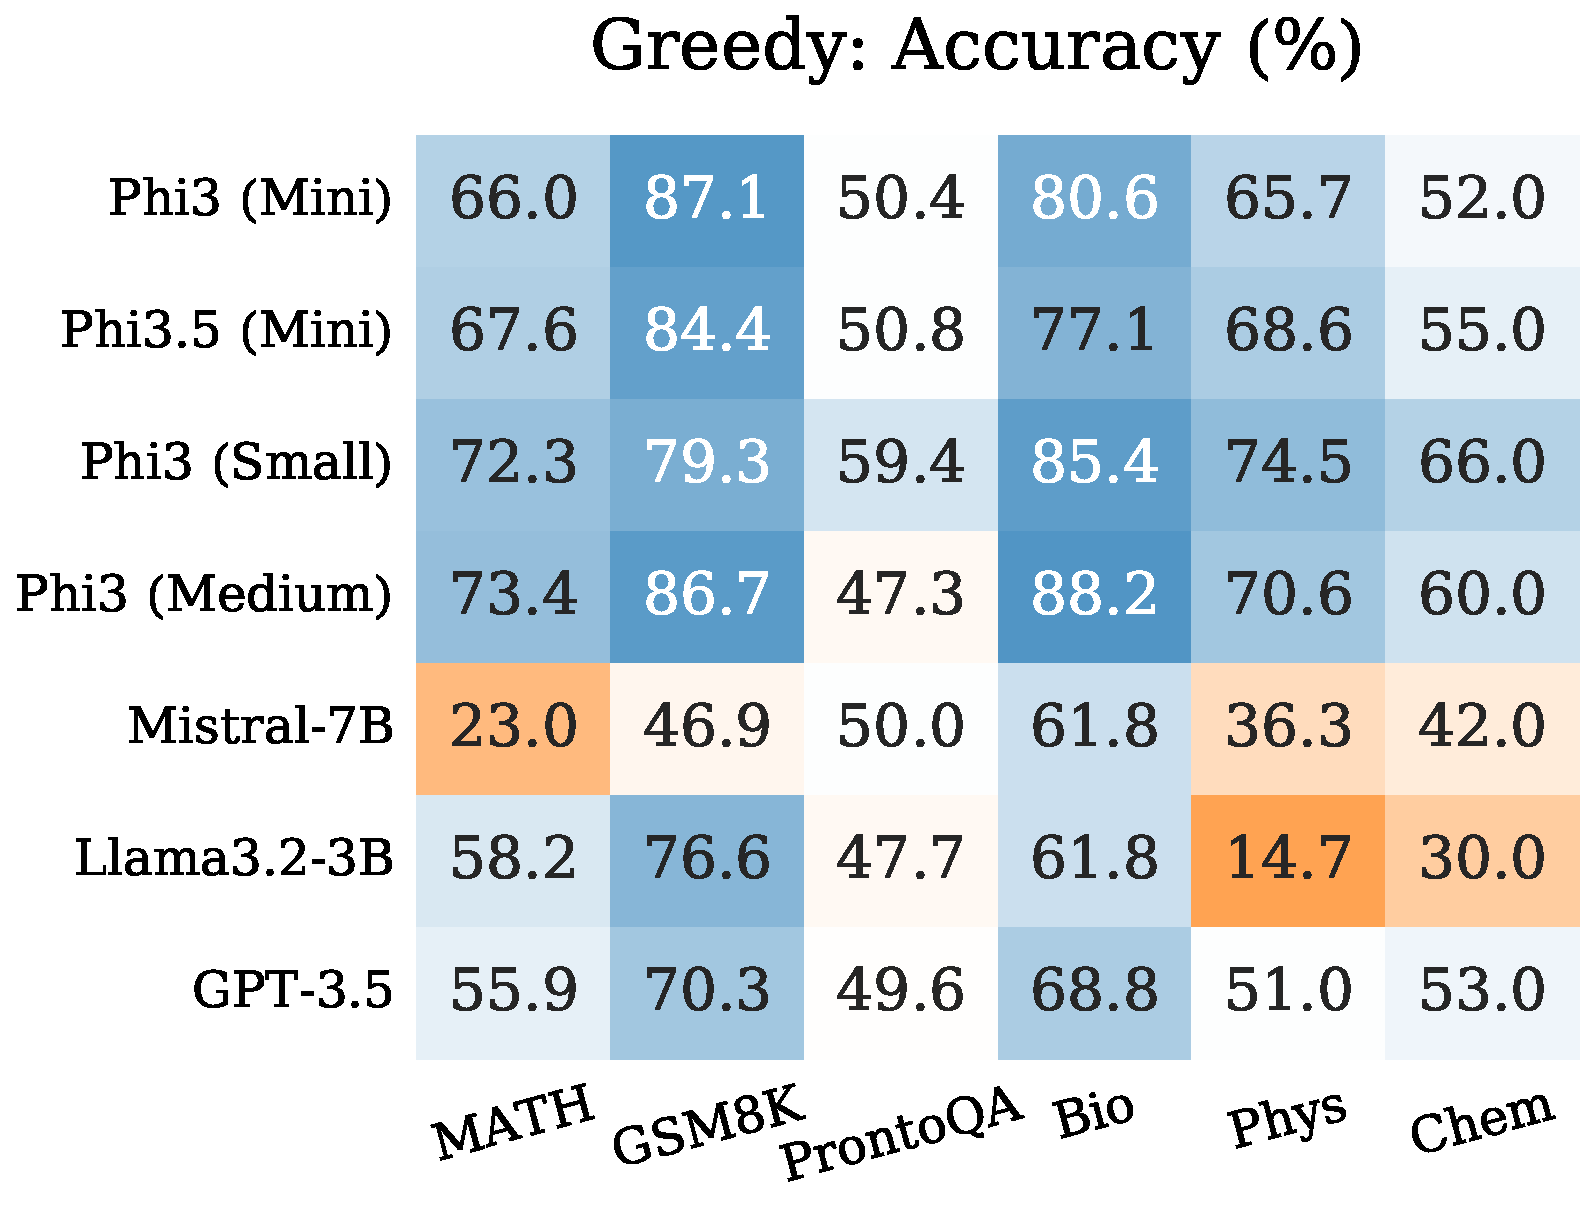
\includegraphics[width=0.45\textwidth]{figs/BoN-greedy-Colored-Table.pdf}
        \label{sfig:bon-greedy}
    }
    
    
    \caption{Performance of alternative self-reward functions for inference-time BoN sharpening:  Percent accuracy improvement over greedy decoding for (a) BoN sharpening with length-normalized log probability and (b) majority voting, with both demonstrating efficacy on a range of model-task pairs.  (c) Coverage of correct answer, a skyline demonstrating that most model-task pairs produce the correct answer in at least one completion out of 50 for most prompts.  (d) Accuracy of greedy decoding baseline on each model-task pair.
    }
    \label{fig:other_rewards}
  \end{figure}

\subsection{Training-Time Sharpening with \bestofnalg}
\begin{table}[t]
    \centering
    \begin{tabular}{cccc}
        \toprule
        \textbf{Model} & \textbf{Dataset} & \textbf{\% Lift over Greedy (Accuracy)} & \textbf{Lift over Greedy (Likelihood)} \\
        \midrule
        \phithreefivemini & \mathdataset & $19.24 \pm 2.41$ & $48.33 \pm 0.17$ \\
        \phithreefivemini & \gsm & $1.82 \pm 0.64$ & $1.49 \pm 0.55$ \\
        \phithreefivemini & \prontoqa & $12.46 \pm 1.08$ & $ 5.64 \pm 0.01$ \\
        \texttt{Mistral-7B} & \mathdataset & $8.88 \pm 5.55$ & $5.71 \pm 3.00$ \\
        \bottomrule
    \end{tabular}
    \caption{Experimental results for \bestofnalg}
    \label{tab:performance}
\end{table}
In addition to inference-time experiments, we also evaluate training-time sharpening, and demonstrate empirically that \bestofnalg effectively amortizes inference-time BoN.  Due to limited computational resources, we restrict our attention to a subset of the model-task pairs considered in \Cref{ssec:inference} that have particularly promising inference-time BoN performance. For each pair, we evaluate the performance of \bestofnalg as a means to amortize the inference-time cost of multiple generations.

For each of the chosen model-dataset pairs (cf. \Cref{tab:performance}), we sample $N=50$ responses with temperature 1 for each prompt in the dataset and select the most likely (according to the relevant reference model).  We then combine these likely responses with the prompts in order to form a training corpus and train with the \bestofnalg objective. We apply Low Rank Adaptation \citep{hu2021lora} to the model, sweeping over LoRA rank, learning rate scheduler, and weight decay in order to return the best optimized model.\footnote{In all experiments involving \phithreefivemini we use a batch size of 4; unfortunately, due to a known numerical issue with LoRA on \mistral involving batch size $>1$, we use a batch of 1 in this case.  Because of this choice, instead of the 30 epochs we use to train our other models, for \mistral, we run only 10 epochs.}  We report the specific hyperparameters chosen in \Cref{tab:hyperparameters}.  On all models, we used a learning rate of $3 \times 10^{-4}$ with linear decay to zero and gradient clamping at 0.1. \loose

\paragraph{Results}  \Cref{tab:performance} reports our results for \bestofnalg. We report best model checkpoint during training for each model-dataset pair, averaged across 3 random seeds, with responses are sampled with temperature 1 from the fine-tuned model.  We report (i) the percent lift in accuracy on the dataset with respect to the greedy generation of the reference model; and (ii) the increase in average sequence level log-likelihood with respect to the same. For all model-dataset pairs, we observe improvement on both metrics, demonstrating that some amortization is possible with \bestofnalg.

Next, in \Cref{fig:training_curve_phi,fig:training_curve_mistral} (\cref{sec:additional_experiments}), we display the evolution of the metrics in \cref{tab:performance} throughout training for each model-dataset pair.  In \cref{fig:training_curve_phi}, we find that while \phithreefivemini is quite well-behaved on \mathdataset and \prontoqa, the training curve for \gsm is quite noisy. The log-probability appears to be a significantly less useful proxy for accuracy on this dataset than for the others; similar phenomena were observed in \citet{block2023butterfly} in a variety of tasks.  In \cref{fig:training_curve_mistral}, we find that for \mistral on \mathdataset, we achieve improvement after training for sufficiently long, but the optimization suffers an substantial initial drop and spends $\sim90\% $ of the gradient steps recovering before improvement is observed; we speculate that this is a function of insufficient hyper-parameter tuning for the optimization itself, rather than a fundamental barrier.

Finally, in \Cref{fig:sft-N} (\cref{sec:additional_experiments}), we investigate the effect of the parameter $N$ on the performance of \bestofnalg for \phithreefivemini on \mathdataset.  In particular, in forming our training set, we choose $N \in \{10, 25, 50 \}$ and repeat the procedure described above, averaging our results over three seeds.  We find that increasing $N$ leads to a modest increase in the sequence-level log-likelihood, in accordance with our theory, and a consequent increase in the accuracy of the fine-tuned model.


